\documentclass[11pt,a4paper]{article}

\usepackage[T1]{fontenc}
\usepackage[utf8]{inputenc}
\usepackage{lmodern}
\usepackage[margin=1in]{geometry}
\usepackage{amsmath,amssymb,mathtools,bm}
\usepackage{booktabs}
\usepackage{array}
\usepackage{tocloft}
\usepackage{hyperref}
\usepackage{enumitem}
\usepackage{xcolor}
\usepackage{tikz}
\usetikzlibrary{arrows.meta,positioning,shapes.geometric}

\hypersetup{
  colorlinks=true,
  linkcolor=blue!55!black,
  urlcolor=blue!55!black,
  citecolor=blue!55!black,
  linktoc=all,
  pdftitle={Inverted Pendulum Control Game - Technical Documentation}
}

\title{\textbf{Inverted Pendulum Control Game}\\Comprehensive Technical Documentation}
\author{Project: \texttt{cart\_pole\_control\_game}}
\date{\today}

\newcommand{\state}{\mathbf{x}}
\newcommand{\A}{\mathbf{A}}
\newcommand{\B}{\mathbf{B}}
\newcommand{\Q}{\mathbf{Q}}
\newcommand{\R}{\mathbf{R}}

% Increase TOC spacing so entries distribute across pages 2 and 3.
\setlength{\cftbeforesecskip}{15pt}
\setlength{\cftbeforesubsecskip}{2.8pt}

\begin{document}
\pagenumbering{gobble}
\begin{titlepage}
  \centering
  \vspace*{\fill}
  {\LARGE\bfseries Inverted Pendulum Control Game\par}
  \vspace{0.8em}
  {\Large Comprehensive Technical Documentation\par}
  \vspace{1.8em}
  {\large Project: \texttt{cart\_pole\_control\_game}\par}
  \vspace{0.8em}
  {\large \today\par}
  \vspace*{\fill}
\end{titlepage}
\clearpage
\pagenumbering{arabic}
\setcounter{page}{3}
\tableofcontents
\clearpage

\section{Project Purpose and Scope}
This project is an in-browser, zero-dependency control-theory simulator for an inverted pendulum on a cart (cart-pole). It compares three classical control strategies in real time:
\begin{enumerate}[label=\arabic*.]
  \item PID (dual-loop parallel form),
  \item LQR (linear-quadratic regulator on a linearized model),
  \item MPC (finite-horizon nonlinear shooting with gradient descent).
\end{enumerate}

The simulator integrates nonlinear dynamics with RK4, renders all telemetry on a canvas UI, allows live gain tuning, and logs per-tick data for download.

\section{Why the Inverted Pendulum?}
The inverted pendulum is a canonical benchmark for feedback control because:
\begin{enumerate}[label=\arabic*.]
  \item It is open-loop unstable around the upright equilibrium.
  \item It is nonlinear and coupled (cart position and pole angle are dynamically linked).
  \item It has practical constraints (force limits, track limits), mirroring real systems.
  \item It cleanly demonstrates differences between model-free feedback (PID), optimal linear control (LQR), and constrained predictive control (MPC).
\end{enumerate}

\section{System Modeling}
\subsection{State, Input, and Sign Convention}
The simulator uses the state vector
\begin{equation}
\state = \begin{bmatrix}x & \dot{x} & \theta & \dot{\theta}\end{bmatrix}^\top,
\end{equation}
where:
\begin{enumerate}[label=\arabic*.]
  \item $x$: cart position,
  \item $\dot{x}$: cart velocity,
  \item $\theta$: pole angle from \emph{upright} ($\theta=0$ is perfectly upright),
  \item $\dot{\theta}$: angular velocity.
\end{enumerate}

Control input:
\begin{equation}
u = \text{horizontal force applied to the cart (N)}.
\end{equation}

In this implementation, a positive angle (pole leaning right) requires a positive corrective push (cart pushed right) to move under the pole.

\subsection{Physical Parameters}
Default parameters are loaded from \texttt{js/config.js}.

\begin{center}
\begin{tabular}{>{\ttfamily}l c l}
\toprule
Symbol & Default & Meaning \\
\midrule
$M$ & 1.0 & cart mass (kg) \\
$m$ & 0.3 & pole mass (kg) \\
$L$ & 0.6 & pole half-length parameter (m) \\
$g$ & 9.81 & gravity (m/s\textsuperscript{2}) \\
$b$ & 0.1 & cart viscous friction coefficient \\
$U_{\max}$ & 30 & actuator limit used by controllers (N) \\
$dt_{\text{inner}}$ & 0.002 & physics sub-step (s), nominal 500 Hz \\
\bottomrule
\end{tabular}
\end{center}

\subsection{Nonlinear Dynamics Used in Code}
Dynamics are implemented in \texttt{js/physics.js} as:
\begin{align}
D(\theta) &= M + m\sin^2\theta, \\
\ddot{x} &= \frac{u - b\dot{x} + mL\dot{\theta}^2\sin\theta + mg\sin\theta\cos\theta}{D(\theta)}, \\
\ddot{\theta} &= \frac{-(M+m)g\sin\theta - \cos\theta\left(u - b\dot{x} + mL\dot{\theta}^2\sin\theta\right)}{L D(\theta)}.
\end{align}
Thus the state derivative is
\begin{equation}
\dot{\state} = f(\state, u) =
\begin{bmatrix}
\dot{x} \\
\ddot{x} \\
\dot{\theta} \\
\ddot{\theta}
\end{bmatrix}.
\end{equation}

\subsection{Lagrangian Background (Conceptual)}
These equations are the standard cart-pole Lagrange equations in manipulated form:
\begin{equation}
\frac{d}{dt}\left(\frac{\partial \mathcal{L}}{\partial \dot{q}_i}\right) -
\frac{\partial \mathcal{L}}{\partial q_i} = Q_i,
\end{equation}
with generalized coordinates $q=\{x,\theta\}$, $\mathcal{L}=T-V$, and generalized force on cart equal to $u-b\dot{x}$.

\section{Numerical Simulation and Constraints}
\subsection{Integration}
The continuous dynamics are integrated using fourth-order Runge--Kutta (RK4):
\begin{equation}
\state_{k+1} = \text{RK4}\!\left(\state_k,u_k,\Delta t\right).
\end{equation}

At render frame time, the simulator computes a frame $\Delta t$ and subdivides it into many physics sub-steps near $dt_{\text{inner}}=0.002$ s.

\subsection{Applied Input and Saturation}
At each frame:
\begin{enumerate}[label=\arabic*.]
  \item Controller computes $u$.
  \item Manual push / challenge disturbance is added.
  \item Final input is clamped in \texttt{main.js} to
  \begin{equation}
  u \in [-1.5U_{\max},\,1.5U_{\max}].
  \end{equation}
\end{enumerate}

Inside MPC rollout and MPC cost evaluation, each candidate control is clamped to
\begin{equation}
u_k \in [-U_{\max},U_{\max}].
\end{equation}

\subsection{Track Boundary and Failure Condition}
\begin{enumerate}[label=\arabic*.]
  \item Soft track wall: when $|x|$ exceeds \texttt{trackLen}, velocity is damped and position clamped.
  \item Episode fails when
  \begin{equation}
  |\theta| > 0.65\pi \approx 117^\circ.
  \end{equation}
\end{enumerate}

\section{Linearization About Upright}
\subsection{Linear Model}
The project linearizes at the upright equilibrium:
\begin{equation}
\theta=0,\quad \dot{x}=0,\quad \dot{\theta}=0,\quad u=0.
\end{equation}

Resulting continuous-time linear model:
\begin{equation}
\dot{\state} = \A \state + \B u,
\end{equation}
with
\begin{equation}
\A =
\begin{bmatrix}
0 & 1 & 0 & 0 \\
0 & -b/M & mg/M & 0 \\
0 & 0 & 0 & 1 \\
0 & b/(LM) & -(M+m)g/(LM) & 0
\end{bmatrix},
\quad
\B =
\begin{bmatrix}
0 \\ 1/M \\ 0 \\ -1/(LM)
\end{bmatrix}.
\end{equation}

\subsection{Interpretation}
This linearization is accurate near upright and is used by LQR for analytic gain synthesis. MPC uses the \emph{nonlinear} model for prediction.

\section{PID Controller in This Project}
\subsection{Classical PID}
For tracking error $e(t)$, ideal PID is
\begin{equation}
u(t)=K_P e(t)+K_I\int_0^t e(\tau)d\tau + K_D\frac{de(t)}{dt}.
\end{equation}

\subsection{Project-Specific Dual-Loop PID Law}
This project uses two coupled PID-like loops with state feedback:
\begin{align}
u_\theta &= K_{p\theta}\theta + K_{i\theta}\!\int\theta\,dt + K_{d\theta}\dot{\theta},\\
u_x &= -\left(K_{px}x + K_{ix}\!\int x\,dt + K_{dx}\dot{x}\right),\\
u &= u_\theta + u_x.
\end{align}

Default gains:
\begin{equation}
\{K_{p\theta},K_{i\theta},K_{d\theta},K_{px},K_{ix},K_{dx},i_{\max}\}
=\{64,2,9.8,10,0.5,15.3,8\}.
\end{equation}

\subsection{Anti-Windup and Initialization}
Integral states are clamped each tick:
\begin{align}
I_\theta &\leftarrow \text{clip}(I_\theta + \theta\,dt,\,-i_{\max},\,i_{\max}),\\
I_x &\leftarrow \text{clip}(I_x + x\,dt,\,-i_{\max},\,i_{\max}).
\end{align}
On first call after reset/mode switch, PID returns $u=0$ once (\texttt{\_pidNeedsInit}) to avoid transients from stale integral state.

\subsection{Algorithmic Nature}
PID in this code does \emph{not} solve an optimization problem and does not use a numerical solver for gains online. It evaluates algebraic formulas each frame: computational cost $O(1)$.

\section{LQR Controller in This Project}
\subsection{Optimal Control Problem}
For linearized dynamics $\dot{\state}=\A\state+\B u$, continuous-time infinite-horizon LQR minimizes:
\begin{equation}
J=\int_0^\infty \left(\state^\top\Q\state + u^\top\R u\right)dt,
\end{equation}
with
\begin{equation}
\Q=\text{diag}(Q_x,Q_{\dot{x}},Q_\theta,Q_{\dot{\theta}}),\quad \R=[R].
\end{equation}

Defaults:
\begin{equation}
\Q=\text{diag}(1,0.8,20,2.5),\quad R=0.01.
\end{equation}

\subsection{CARE and Feedback Law}
LQR gain is obtained from continuous-time algebraic Riccati equation (CARE):
\begin{equation}
\A^\top P + P\A - P\B\R^{-1}\B^\top P + \Q = 0,
\end{equation}
then
\begin{equation}
K=\R^{-1}\B^\top P,\qquad u=-K\state.
\end{equation}

\subsection{How CARE Is Solved Here}
This project uses a custom iterative integration of the Riccati differential equation toward steady state:
\begin{equation}
\dot{P} = \A^\top P + P\A - P\B\R^{-1}\B^\top P + \Q.
\end{equation}
Implementation details:
\begin{enumerate}[label=\arabic*.]
  \item Initialize $P_0=\text{diag}(Q_x,Q_{\dot{x}},Q_\theta,Q_{\dot{\theta}})$.
  \item Euler update $P \leftarrow P + dt\cdot \dot{P}$ with $dt=10^{-4}$.
  \item Stop when $\|\dot{P}\|_F$ is sufficiently small (or max iterations reached).
\end{enumerate}

This is a custom numeric solver in \texttt{js/lqr.js}; no external linear algebra library is used.

\subsection{Closed-Loop Eigenvalues (Display)}
For display only, the code computes eigenvalues of
\begin{equation}
\A_{\text{cl}} = \A - \B K
\end{equation}
by:
\begin{enumerate}[label=\arabic*.]
  \item Building characteristic polynomial via Newton identities.
  \item Solving degree-4 polynomial roots using Durand--Kerner.
\end{enumerate}

This verifies stability ($\Re\{\lambda_i\}<0$).

\subsection{Runtime Policy and Live Recompute}
\begin{enumerate}[label=\arabic*.]
  \item Startup: solve LQR once, store \texttt{sim.lqrData}.
  \item Runtime: each tick applies $u=-K\state$ in $O(1)$.
  \item Tuner changes to $Q/R$: trigger debounced re-solve after 120 ms.
\end{enumerate}

\section{MPC Controller in This Project}
\subsection{Optimization Problem}
This is receding-horizon nonlinear MPC with direct shooting over control sequence
\begin{equation}
U=\{u_0,\ldots,u_{N_h-1}\}.
\end{equation}

Cost implemented in \texttt{mpcCost}:
\begin{equation}
J(U)=\sum_{k=0}^{N_h-1}\left(
Q_x x_k^2 + Q_{\dot{x}}\dot{x}_k^2 + Q_\theta \theta_k^2 + Q_{\dot{\theta}}\dot{\theta}_k^2 + R u_k^2
\right)
 + Q_f\!\left(Q_x x_N^2 + Q_{\dot{x}}\dot{x}_N^2 + Q_\theta \theta_N^2 + Q_{\dot{\theta}}\dot{\theta}_N^2\right),
\end{equation}
with $Q_f=15$.

Dynamics constraint in prediction:
\begin{equation}
\state_{k+1}=f_{\text{RK4}}(\state_k,u_k,dt_{\text{MPC}}),\quad u_k\in[-U_{\max},U_{\max}].
\end{equation}

\subsection{Horizon Definitions}
\begin{enumerate}[label=\arabic*.]
  \item Prediction horizon steps: $N_h=22$ (default).
  \item MPC time step: $dt_{\text{MPC}}=0.025$ s.
  \item Look-ahead duration: $N_h dt_{\text{MPC}}=0.55$ s.
  \item State horizon: $N_h+1$ states ($x_0$ to $x_{N_h}$).
  \item Control horizon: $N_h$ (all horizon controls are optimized).
\end{enumerate}

\subsection{Solver Used Here}
This MPC uses a \textbf{custom finite-difference batch gradient-descent shooting solver}:
\begin{enumerate}[label=\arabic*.]
  \item Warm start:
  \begin{enumerate}[label*=\arabic*.]
    \item first call or reset: seed sequence by rolling out LQR policy,
    \item subsequent calls: shift old sequence left (receding horizon), copy tail.
  \end{enumerate}
  \item For each iteration ($N_i=12$ default):
  \begin{enumerate}[label*=\arabic*.]
    \item compute base cost $J_0$,
    \item for each index $k$, perturb $u_k$ by $\epsilon=1.0$ and estimate
    \begin{equation}
    \frac{\partial J}{\partial u_k}\approx \frac{J(U+\epsilon e_k)-J(U)}{\epsilon},
    \end{equation}
    \item batch update all controls:
    \begin{equation}
    u_k \leftarrow \text{clip}(u_k - \eta g_k,\,-U_{\max},U_{\max}),\quad \eta=0.5.
    \end{equation}
  \end{enumerate}
  \item Apply only $u_0$ to plant; keep $u_1,\ldots,u_{N_h-1}$ for next frame.
\end{enumerate}

\subsection{Online Complexity}
Finite-difference MPC here is approximately $O(N_h^2 N_i)$ due repeated horizon rollouts per gradient component.

\subsection{MPC Output to UI}
Current optimized sequence is also rolled out in \texttt{mpcPredict} and drawn as a ghost trajectory, making the prediction visible in the canvas.

\section{Controller Data Path and ``Instant Responsiveness''}
All controller code, physics, and rendering live in the same browser JS runtime (no backend). Responsiveness comes from shared in-memory state updated every animation frame.

\subsection{Runtime Pipeline}
\begin{center}
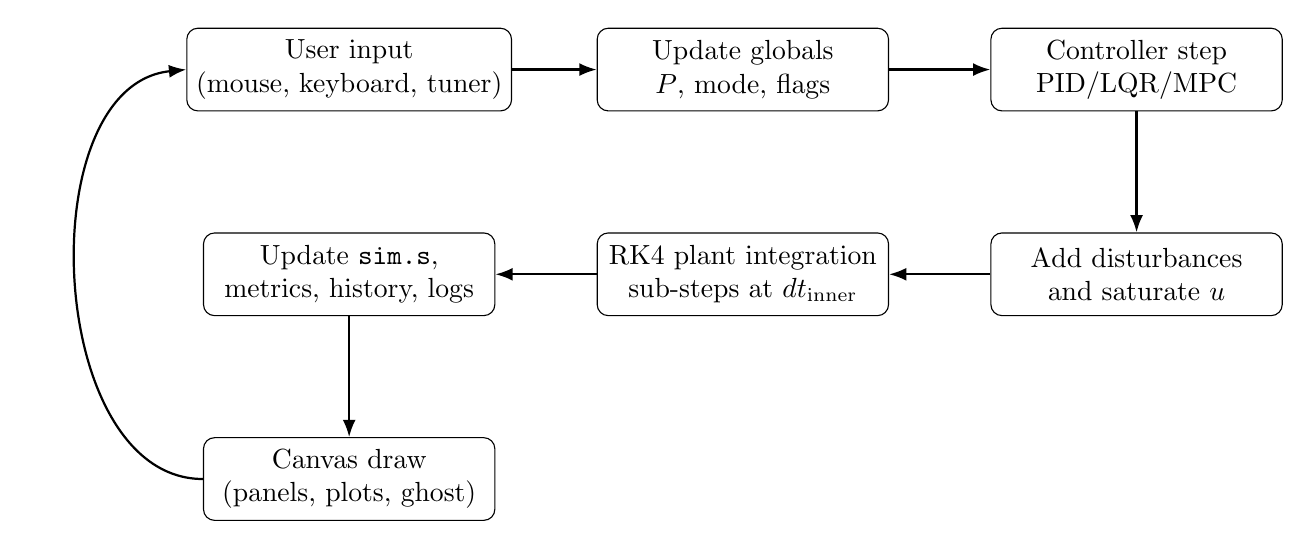
\begin{tikzpicture}[
  box/.style={draw, rounded corners, align=center, minimum width=3.7cm, minimum height=1.05cm},
  arr/.style={-{Latex[length=2.2mm]}, thick}
]
\node[box] at (0,0)   (input) {User input\\(mouse, keyboard, tuner)};
\node[box] at (5.0,0) (params) {Update globals\\$P$, mode, flags};
\node[box] at (10.0,0) (ctrl) {Controller step\\PID/LQR/MPC};
\node[box] at (10.0,-2.6) (sat) {Add disturbances\\and saturate $u$};
\node[box] at (5.0,-2.6) (plant) {RK4 plant integration\\sub-steps at $dt_{\text{inner}}$};
\node[box] at (0,-2.6) (state) {Update \texttt{sim.s},\\metrics, history, logs};
\node[box] at (0,-5.2) (draw) {Canvas draw\\(panels, plots, ghost)};

\draw[arr] (input) -- (params);
\draw[arr] (params) -- (ctrl);
\draw[arr] (ctrl) -- (sat);
\draw[arr] (sat) -- (plant);
\draw[arr] (plant) -- (state);
\draw[arr] (state) -- (draw);
\draw[arr] (draw.west) .. controls +(-2.0,0.0) and +(-2.0,-0.2) .. (input.west);
\end{tikzpicture}
\end{center}

\subsection{Per-Controller Gain/Action Update Path}
\paragraph{PID}
Tuner slider directly edits \texttt{P.pid.*}; next \texttt{tick()} uses new gains immediately.

\paragraph{LQR}
Tuner edits $Q/R$ then debounced \texttt{solveLQR()} recomputes $K$ and stores \texttt{sim.lqrData}; next tick applies new $u=-Kx$.

\paragraph{MPC}
Tuner edits $Q/R/N_h$ and sets \texttt{\_mpcNeedsInit}; next \texttt{mpcStep()} reseeds/re-optimizes sequence and applies new $u_0$.

\section{Metrics, Logging, and Visualization}
\subsection{Metrics}
For each controller mode, the simulator tracks:
\begin{enumerate}[label=\arabic*.]
  \item balance time,
  \item settling time (angle below threshold for required duration),
  \item peak $|\theta|$,
  \item control effort $\int u^2 dt$ (numerical accumulation).
\end{enumerate}

\subsection{CSV Logging}
Every simulation tick logs:
\begin{equation}
\texttt{run, t, x, xdot, theta\_rad, thetadot, u, alive}.
\end{equation}

\subsection{Rendered Technical Panels}
The UI displays:
\begin{enumerate}[label=\arabic*.]
  \item current state vector and force,
  \item linearized matrices $\A,\B$,
  \item closed-loop eigenvalues for LQR,
  \item angle history plot,
  \item control history plot,
  \item phase portrait $(\theta,\dot{\theta})$,
  \item controller comparison table,
  \item MPC predicted ghost trajectory.
\end{enumerate}

\section{File-Level Architecture}
\begin{center}
\begin{tabular}{>{\ttfamily}p{3.4cm} p{10.2cm}}
\toprule
File & Responsibility \\
\midrule
index.html & Entry point, script load order, loading overlay, tuner init. \\
js/config.js & Global parameter object \texttt{P}. \\
js/physics.js & Nonlinear dynamics, RK4 integrator, linearization matrices. \\
js/lqr.js & CARE iterative solver, $K$ synthesis, eigenvalue utilities. \\
js/mpc.js & Receding-horizon MPC with finite-difference gradient descent. \\
js/pid.js & Dual-loop PID and anti-windup integrator state. \\
js/main.js & Simulation state, tick/frame loop, integration, metrics, logs. \\
js/render.js & Full canvas rendering for desktop and mobile layouts. \\
js/interaction.js & Keyboard/mouse/touch handling and mode switching. \\
js/tuner.js & Floating live tuner UI and live parameter update logic. \\
css/style.css & Global page/canvas styling and loading overlay style. \\
css/tuner.css & Tuner panel styling and responsive behavior. \\
\bottomrule
\end{tabular}
\end{center}

\section{Known Implementation Notes}
\begin{enumerate}[label=\arabic*.]
  \item The runtime app is the modular stack loaded by \texttt{index.html}; the file \texttt{cartpole} is a standalone legacy snapshot and is not the active entrypoint.
  \item Keyboard binding for PID switch in code is \texttt{KeyI}; if documentation says \texttt{P} for PID, that is inconsistent with current implementation.
  \item \texttt{mpcU} is allocated once using initial \texttt{P.Nh}; increasing \texttt{Nh} above startup value without reallocating can lead to invalid MPC values.
\end{enumerate}

\clearpage
\section{Practical Comparison of Controllers in This Project}
\begin{center}
\begin{tabular}{>{\raggedright\arraybackslash}p{2.5cm} p{4.2cm} p{4.1cm} p{3.8cm}}
\toprule
Controller & Mathematical basis & Online computation & Strengths/limits here \\
\midrule
PID & Heuristic feedback + integral memory & $O(1)$ & Simple and robust; no model-based optimality or explicit constraints. \\
LQR & Linear optimal control from CARE & $O(1)$ & Very efficient; optimal for linearized model, less accurate far from upright. \\
MPC & Finite-horizon nonlinear optimization & Heavy ($O(N_h^2N_i)$ approx.) & Handles nonlinear rollout and constraints directly; higher compute cost. \\
\bottomrule
\end{tabular}
\end{center}

\section*{Conclusion}
This project is a compact but technically rich control-systems lab. It combines:
\begin{enumerate}[label=\arabic*.]
  \item nonlinear plant simulation,
  \item linear model-based optimal control (LQR),
  \item nonlinear constrained predictive optimization (MPC),
  \item practical feedback design (PID),
  \item live interactive visualization and tuning.
\end{enumerate}
As implemented, it is ideal for studying controller trade-offs between simplicity, optimality assumptions, and real-time computational cost.

\end{document}
